\subsection{Komplexe Datenstrukturen}
\subsubsection{XML}
XML ist eine Abkürzung für Extensible Markup Language, die im Jahr 1998 erfinden wurde. der Herr. Helmut Vonhoegen definiert der XML als erste frei verfügbares Format für strukturierte Daten, unabhängig von bestimmten Plattformen und Anwendungen. Auch als Format für den Datenaustausch etabliert. XML ist auch ein universelles Datenbeschreibungsformat, weil es als einer der Web-Standards gilt, die vom W3C standardisiert wurden, weil es eine bessere Strukturierung des Dokuments ermöglicht und es auch erlaubt, die Dokumente im Web zu tauchen, was seine Besonderheit ausmacht. Die XML ist wegen ihrer Einfachheit sehr nützlich, aber auch, weil sie unabhängig von jeder Plattform, Anwendung, Kodierung, Protokoll usw. ist. Um XML besser zu verstehen, ist es wichtig, einen Blick in seine Vergangenheit zu werfen.

\textit{\textbf{Historik}}

die Sprache XML ist von den beiden Sprachen SGML und HTML abgeleitet. SGML (Standard Generalized Markup Language), der Vorläufer von HTML und XML, war für die Strukturierung von Dokumenten mit Hilfe von Tags gedacht, hatte aber den großen Nachteil, dass es nicht für das Web erweiterbar war und somit die Sprache HTML, um alle Informationen im Web zugänglich zu machen.  HTML ist wie wir alle wissen, eine Sprache, die es erlaubt Seiten zu erstellen, die im Web angezeigt werden können. Aber der Nachteil von HTLM ist, dass es Fakten und Formen vermischt.Als gemeinsamen Punkt können wir festhalten, dass HTML und XML zwei Sprachen sind, die sich am Text orientieren und Tags bilden, die es erlauben, Daten strukturell zu organisieren. Daraus wird XML geboren. 

Die Idee hinter der Schaffung von XML war, etwas zu haben, das Inhalt von Formen trennt und auch über das Web zugänglich ist. Während die Tags in HTML in erster Linie festlegen, in welche Form Inhalte in einem entsprechenden Medium ausgegeben werden sollen, wird mit XML versucht, die Bedeutung von Daten so festzulegen, dass nicht nur Menschen, sondern auch Maschinen damit etwas anfangen können.\cite{helmut32}

\textit{\textbf{Anwendung}}

Um ein syntaktisch korrektes XML-Dokument zu schreiben, müssen zunächst zwei grundlegende Prinzipien beachtet werden. Erstens muss das XML-Dokument wohlgeformt sein (Well form). Das bedeutet, dass erstens die Regeln und Konventionen für das Schreiben der Tags eingehalten werden müssen, die vom W3C vorgegeben werden, und zweitens muss auch die Verschachtelungsreihenfolge der Tags beachtet werden. Das zweite Prinzip ist, dass das XML-Dokument gültig sein muss. Dies ist ein optionaler Schritt, der aber notwendig ist, wenn wir möchten, dass unsere XML-Datei einem Dokumentenmodell folgt.

Die Benützung von XML-Anwendung wird für Auszeichnungssprachen verwendet, die mit Hilfe von XML definiert wurden. Es handelt sich also um XML-Vokabulare oder Dokumenttypen, die für bestimmte Bereich fixiert wurden.\cite{helmut36}
Die folgenden Bilder zeigen zunächst den Aufbau eines XML-Dokuments und danach eine Beispiel-XML-Datei.

\begin{center}
%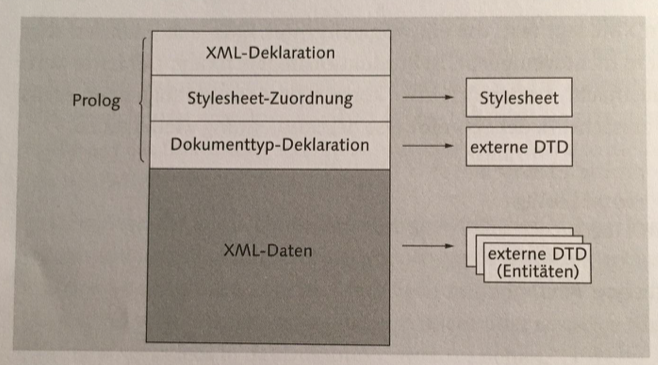
\includegraphics[scale=.5]{./images/8.Aufbauschema_eines_XML-Dockuments}
\captionof{figure}{Aufbauschema eines XML-Dockuments}

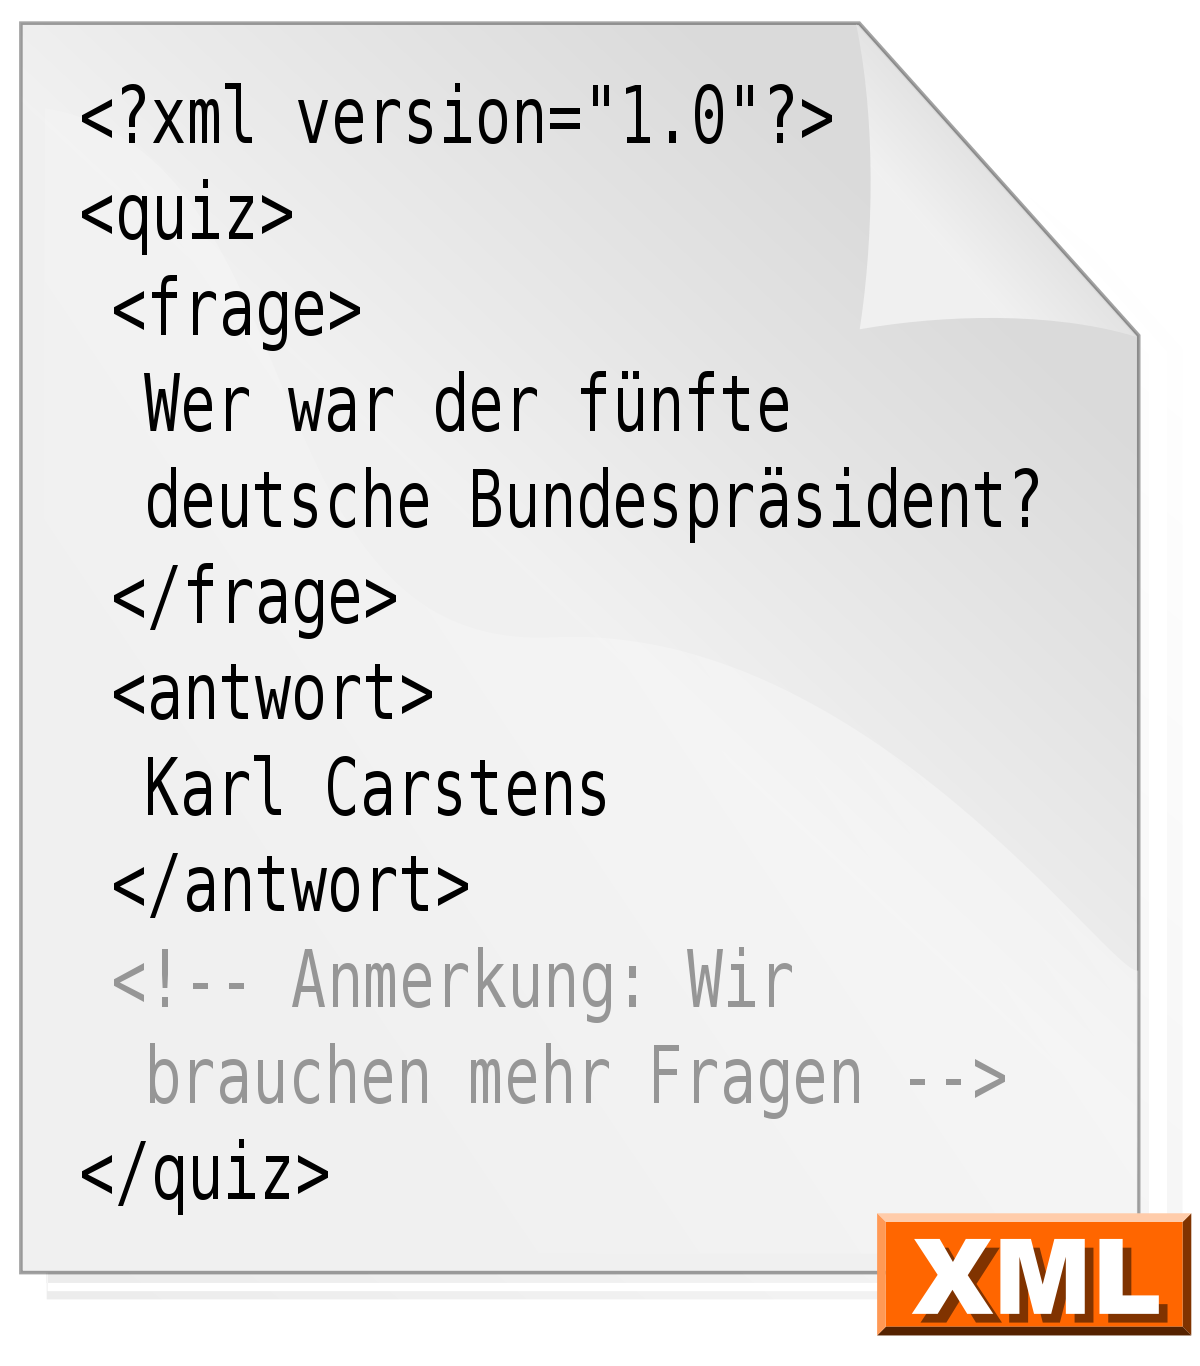
\includegraphics[width=.7\textwidth]{./images/8.Xml_datei_Beispiel}
\captionof{figure}{Beispiel einer XML-Datei}
\end{center}

\subsubsection{JSON}

JSON steht für JavaScript Object Notation und bezeichnet die kompakte Schreibweise von Objekt- und Arraystrukturen.\cite{philipp524} Es handelt sich um ein textuelles Daten Format, das von der Objekt Notation der JavaScript-sprache abgeleitet ist. es wird sehr gerne als Datentransportsprache zwischen Client und Server für Ajax-anfragen verwendet. Für einen schnellen Austausch wird es oft gegenüber XML bevorzugt. Werfen wir zuerst einen Blick auf die Geschichte von JSON. 

\textit{\textbf{Historik}}

Kurz nach Beginn des großen AJAX-Hypes im Jahr 2005 etablierte sich aus praktischen Gründen neben Klartext und XML quasi eine weiteres Übertragungsformat für die Kommunikation via AJAX: JSON, die JavaScript Objekt Notation.\cite{philipp658}
Der JSON wurde von Douglas Crockford zwischen 2002 und 2005 gebaut. Der erste JSON-Standard ist ECMA-404, der im Oktober 20032 veröffentlicht wurde. Derzeit wird er von zwei konkurrierenden Standards beschrieben: IETF RFC 82593 und ECMA-4044. Die neueste Version der Formatspezifikation stammt vom Dezember 2017. \cite{wikip01}

\textit{\textbf{Anwendung}}

Um ein vollständiges und konformes JSON zu erstellen, ist es notwendig, die richtige Syntax zu befolgen und das Dokument mit der Erweiterung .json zu speichern. Ein Json-Objekt beginnt und endet mit geschweiften Klammern {} und besteht im Wesentlichen aus zwei Teilen: Schlüssel und Werte. 

Die Schlüssel sind Zeichenketten, sie enthalten eine Folge von Zeichen, die von Anführungszeichen umgeben sind. Wert ist ein gültiger JSON-Datentyp. Es kann in Form eines Arrays, Objekts, einer Zeichenkette, eines booleschen Wertes, einer Zahl oder null vorliegen. Es kann zwei oder mehr Schlüssel/Wertpaare enthalten, die durch ein Komma getrennt sind. Auf jeden Schlüssel folgt ein Doppelpunkt, um ihn vom Wert zu unterscheiden. Mit diesem Bild ist es möglich, eine Darstellung eines Json zu beobachten. 

\begin{center}
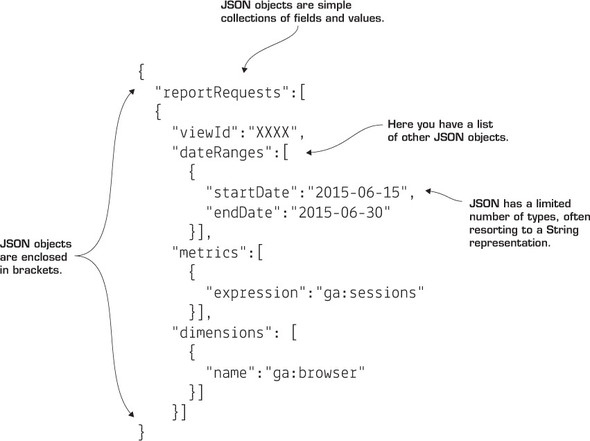
\includegraphics[width=.7\textwidth]{images/8.Darstellung_eines_JSON-Objekts}
\captionof{figure}{Darstellung eines JSON-Objekts}
\end{center}


\subsubsection{BSON}

BSON ist eine Weiterentwicklung des Datenaustauschformates JSON der Firma 10gen und ist unter anderem ein fester Bestandteil von MongoDB. Die Libraries sind für viele Programmiersprachen bereits vorhanden. Da die BSON-Spezifikation öffentlich ist, kann BSON auch für andere Projekte genutzt werden.\cite{thKloeln}

BSON ist so konzipiert, dass es im Raum effektiv ist, aber in einigen Fällen ist es nicht viel effektiver als JSON. In einigen Fällen benötigt BSON sogar mehr Platz als JSON. Der Grund dafür ist ein weiteres Designziel von BSON: die Kreuzbarkeit. BSON fügt den Dokumenten zusätzliche Informationen hinzu, wie z. B. die Länge von Strings und Unterobjekten. Dadurch wird die Traversierung schneller.\cite{bson} BSON ist außerdem so konzipiert, dass es sich schnell kodieren und dekodieren lässt. Ganzzahlen werden z. B. als 32- (oder 64-) Bit-Ganzzahlen gespeichert, so dass sie nicht in und aus dem Text geparst werden müssen. Dies verbraucht mehr Speicherplatz als JSON für kleine ganze Zahlen, aber es ist viel schneller zu parsen. Neben der Kompaktheit fügt BSON zusätzliche Datentypen hinzu, die in JSON nicht verfügbar sind, darunter die Datentypen BinData und Date.“